\chapter{Instrucciones de ejecución}
\label{anx:ejecucion}

En este anexo se describirán las instrucciones para desplegar y operar el prototipo. El código se encuentra en un repositorio público\footnote{Página del repositorio: \url{https://github.com/Starkie/TFM-DistributedAutoadaptiveSystems/tree/main/src/AutoAdaptativeSystem}}. Para seguir estas instrucciones, deberemos clonarlo con \texttt{git} o descargarlo como un fichero zip.

\section{Requisitos}

Para poder ejecutarlo existen los siguientes requisitos. Todos los programas y lenguajes requeridos son compatibles con las principales plataformas (Windows, Linux y Mac).

\begin{itemize}[itemsep=1pt]
  \item SDK de .NET v6.0 o superior\footnote{.NET SDK: \url{https://dotnet.microsoft.com/en-us/download/dotnet/6.0}}.
  \item Docker Compose v2.0 o superior \footnote{Docker compose: \url{https://docs.docker.com/compose/install/}}.
  \item Powershell v5 o Powershell Core\footnote{\url{https://docs.microsoft.com/es-es/powershell/scripting/install/install-other-linux?view=powershell-7.2\#install-as-a-net-global-tool}} (para ejecutar el \foreign{english}{script} de compilación).
  \item Python 3.7 o superior\footnote{Python 3.10: \url{https://www.python.org/downloads/release/python-3106/}} (para generar los API clients).
\end{itemize}

\section{Generar API Clients}

Si se hiciera algún cambio sobre los \foreign{english}{endpoints} que exponen los servicios, tendremos que regenerar los API Clients. Para ello, contamos con un \foreign{english}{script} escrito en Python. Este compila todos los proyectos, genera las especificaciones OpenAPI y, a partir de ellas, genera los clientes.

El \foreign{english}{script} se encuentra en la ruta \texttt{src/AutoAdaptativeSystem/GenerateApiClient.py}. Para ejecutarlo, basta con invocarlo con Python: \texttt{python3 GenerateApiClient.py}. Para que funcione correctamente, todos los proyectos deben encontrarse en un estado compilable.

Si hubiera algún cambio incompatible que haga fallar la compilación, tendremos que corregirlo antes de poder continuar. Por ejemplo, acceder al servicio que falla y solucionar los errores. Hecho esto, podremos ejecutar de nuevo el \foreign{english}{script}. Tendremos que hacer esto hasta que se generen todos los clientes correctamente.

\section{Despliegue}

Para compilar y ejecutar la solución contamos con un \foreign{english}{script} de Powershell. Este se encuentra en la ruta \texttt{src/AutoAdaptativeSystem/build.ps1}. Se encarga de:
\begin{enumerate}
  \item Compilar todos los proyectos de la solución.
  \item Publicar todos los proyectos a una carpeta común.
  \item Crear los contenedores de Docker y levantar la solución con Docker Compose.
\end{enumerate}

Para ejecutarlo, usaremos la instrucción \texttt{pwsh build.ps1}. Si todo ha ido bien, veremos en la consola lo siguiente:

\begin{verbatim}
Container publish-prometheus-1                    Started         3.4s
Container publish-climatisation_monitor-1         Started         1.7s
Container publish-monitoring-1                    Started         2.9s
Container publish-loki-1                          Started         3.4s
Container publish-jaeger-1                        Started         2.5s
Container publish-climatisation_airconditioner-1  Started         1.5s
Container publish-grafana-1                       Started         1.9s
Container publish-rabbitmq-1                      Started         1.7s
Container publish-planning-1                      Started         3.8s
Container publish-climatisation_executor-1       Started         4.2s
Container publish-climatisation_rules-1           Started         4.3s
Container publish-execute-1                       Started         4.2s
Container publish-knowledge-1                     Started         3.5s
Container publish-analysis-1                      Started         4.1s
\end{verbatim}

En cambio, si quisiéramos parar su ejecución, tendremos que acceder a la carpeta \texttt{src/AutoAdaptativeSystem/publish} y ejecutar el comando \texttt{docker-compose down}. Este borrará todas las redes y contenedores que se hayan creado durante el despliegue.

\section{Interactuar con el sistema}

\subsection{Servicios disponibles}

A continuación, se describen algunos de los \foreign{english}{endpoints} más interesantes para interactuar con el sistema (tabla \ref{tab:anx_servicios}). Para consultar la lista completa, puede accederse al fichero \texttt{docker-compose.yml}.

\begin{longtable}{|m{2.3cm}|m{4.6cm}|m{7cm}|}
  \hline

  \textbf{Servicio} & \textbf{\foreign{english}{Endpoint}} & \textbf{Descripción} \\
  \hline

  Grafana & \url{http://localhost:3000} & Acceso a los paneles de monitorización. \\
  \hline

  Climatisation AirConditioner & \url{http://localhost:11001/swagger} & Permite manipular el aire acondicionado y su temperatura actual. \\
  \hline

  Knowledge & \url{http://localhost:5001/swagger} & Permite consultar y manipular las propiedades de adaptación. \\
  \hline
  \caption{Lista de \foreign{english}{endpoints} de interés.}
  \label{tab:anx_servicios}
\end{longtable}

\subsection{Controlar el aire acondicionado}

Para controlar el funcionamiento del aire acondicionado, podemos acceder a la URL correspondiente de la tabla \ref{tab:anx_servicios}. Nos mostrará una pantalla con la lista de operaciones disponibles, similar a la vista en la figura \ref{fig:apis-eps-aireacondicionado}. Nos interesan especialmente las operaciones de \texttt{FakeAirConditioner}. Con ellas podremos simular situaciones distintas para forzar al sistema a adaptarse.

La primera, nos permite cambiar el comportamiento de la temperatura ficticia cuando el dispositivo esté apagado. Se trata del \foreign{english}{endpoint} \texttt{disabled-mode-configuration / \{shouldIncreaseTemperature\}}. Si se le pasa el valor \texttt{true}, la temperatura aumentará. Esto forzará a ejecutar las adaptaciones para enfriar la habitación. Por otro lado, si se le pasa \texttt{false}, la estancia se enfriará y el aparato tendrá que calentarla.

También podemos asignar manualmente la temperatura actual. Con este fin, tenemos el \foreign{english}{endpoint} \texttt{/FakeAirConditioner/temperature}. Así, podrá forzarse la activación de un modo determinado. Aunque permite especificar una unidad, de momento solo están soportadas las temperaturas en grados Celsius.

\subsection{Paneles de monitorización en Grafana}

Para poder visualizar el estado pasado y actual del sistema contamos con el panel de monitorización de Grafana\footnote{Accesible desde \url{http://localhost:3000/d/N0ZSfeUnz/adaptionloop?orgId=1&refresh=10s}}. Al acceder encontraremos algo similar a la figura \ref{anx:apis}. Contaremos con distintas gráficas y visualizaciones de métricas de interés. Por ejemplo, el valor de la temperatura o el tiempo medio de adaptación.

\begin{figure}[h!]
  \centering
  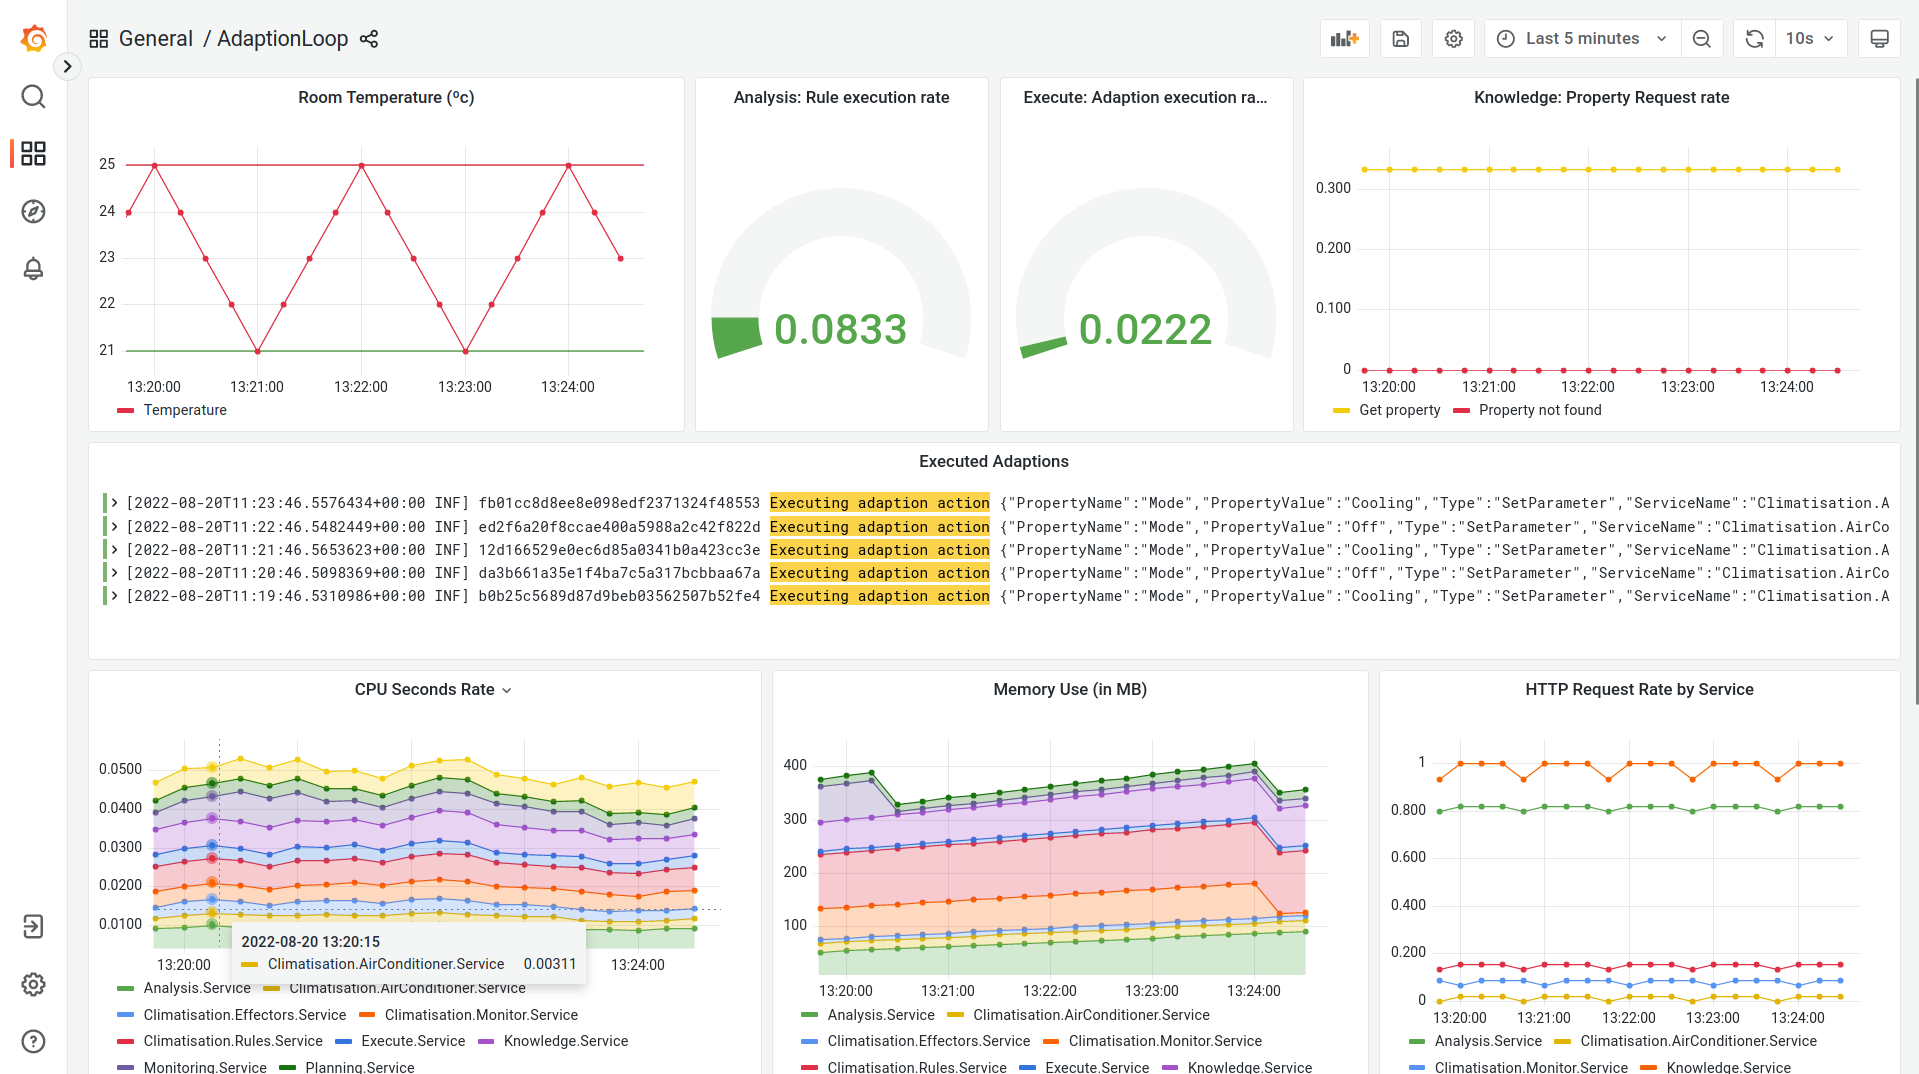
\includegraphics[scale=0.2]{cap_despliegue/images/Grafana-panel-monitorizacion}
  \caption{Panel de monitorización \texttt{AdaptionLoop}.}
  \label{fig:ejecucion-grafana}
\end{figure}

Podemos también explorar las fuentes de datos o ampliarlo con nuevas visualizaciones\footnote{Grafana cuenta con muy buena documentación: \url{https://grafana.com/tutorials/}}. Si queremos hacer cambios y persistirlos para futuras ejecuciones, tendremos que exportar el panel y guardar su contenido en el fichero \texttt{/src/AutoAdaptativeSystem/ config/grafana/dashboards/Adaption-Loop.json}.
